\section{Modeling Metabolites using UKF}
\label{Modeling Metabolites using UKF}




\noindent This is the same system explored in chapter~\ref{chap:EKF_Meskin}, but explored in the context of using an UKF as opposed to an EKF. The original research used an adaptation of the UKF, called the Iterative Unscented Kalman Filter (IUKF), to model the biological pathway of metabolites. Recall that this model contains four different states and 18 unknown parameters. These researchers utilized the IUKF for parameter fitting and was useful in enabling the model converge faster by resetting the covariance to re-excite the model. By not resetting the covariance at this step (as is done in the UKF), the three state variables without measurements converge significantly slower in this model. Utilizing the IUKF on this model was effective, because data regarding metabolites is highly influenced by noise, which is a factor that makes other approaches, such as regression and annealing, fail \cite{article5}. \\ 

\noindent In the paper, researchers had access to their own data sources and used an approach that was adapted from the UKF. Though we are not using their exact dataset, we will be simulating data using the same approach as the previous example. However, this example will be following UKF algorithm, as opposed to the IUKF algorithm. By doing so, the state variables without incoming measurements converge significantly slower than the measurable states. Ultimately, the goal of this example is to demonstrate how the UKF works on higher dimensional and more complex systems and how the UKF can be utilized in parameter estimation. \\

\noindent Recall that the four metabolites have the following differential equations:
\begin{align*}
\dot x_1 &= \alpha_1 x_3^{g_{13}} - \beta_1 x_1^{h_{11}}, \\
\dot x_2 &= \alpha_2 x_1^{g_{21}} - \beta_2 x_2^{h_{22}}, \\
\dot x_3 &= \alpha_3 x_2^{g_{32}} - \beta_3 x_3^{h_{33}} x_4^{h_{34}}, \\
\dot x_4 &= \alpha_4  x_1^{g_{41}} - \beta_4 x_4^{h_{44}},
\end{align*}
with 17 parameters ($\alpha_1, \hdots, \alpha_4, \beta_1, \hdots, \beta_4, g_{13}, g_{21}, g_{32}, g_{41}, h_{11}, h_{22}, h_{33}, h_{34},h_{44} $). In both the original example as well as this one, sampling time will be 0.1 seconds for 5 seconds, totaling 50 UKF estimates. Recall that data is simulated on MATLAB and the model is initialized with state variable $x_0 = [4, 1, 3, 4]^T$ and the state covariance to $P_0 = .01I$. \\

\noindent In the original example, researchers used the following hyper-parameter values: $\epsilon = 1, \kappa = -14$. In theory, values of $\kappa$ can be negative, but negative hyper-parameter values cannot be inputted into MATLAB. For this example, the hyper-parameter values used in this example are set to Matlab default values ($\alpha = 1e-3, \beta = 2, \kappa = 0$). The performance of the UKF on this system with these default hyper parameter values is shown in Figure ~\ref{fig:UKF_states}. Future work includes looking into ways to tune this hyper-parameters. \\

\comment{
\noindent Since the first state, $x1$ is the only state that has incoming system measurements, we have a 3 different blue lines in this figure. From this figure, it appears that the UKF prediction perfectly overlaps with the measured values. However, upon closer inspection, it actually does not. This is likely because there is only a small amount of measurement noise to the system. Figure 4.9 highlights the same information as Figure 4.8, but separates the states into different graphs, enabling a clearer illustration of each state's behavior.
}

\begin{figure}[ht]
    \centering
    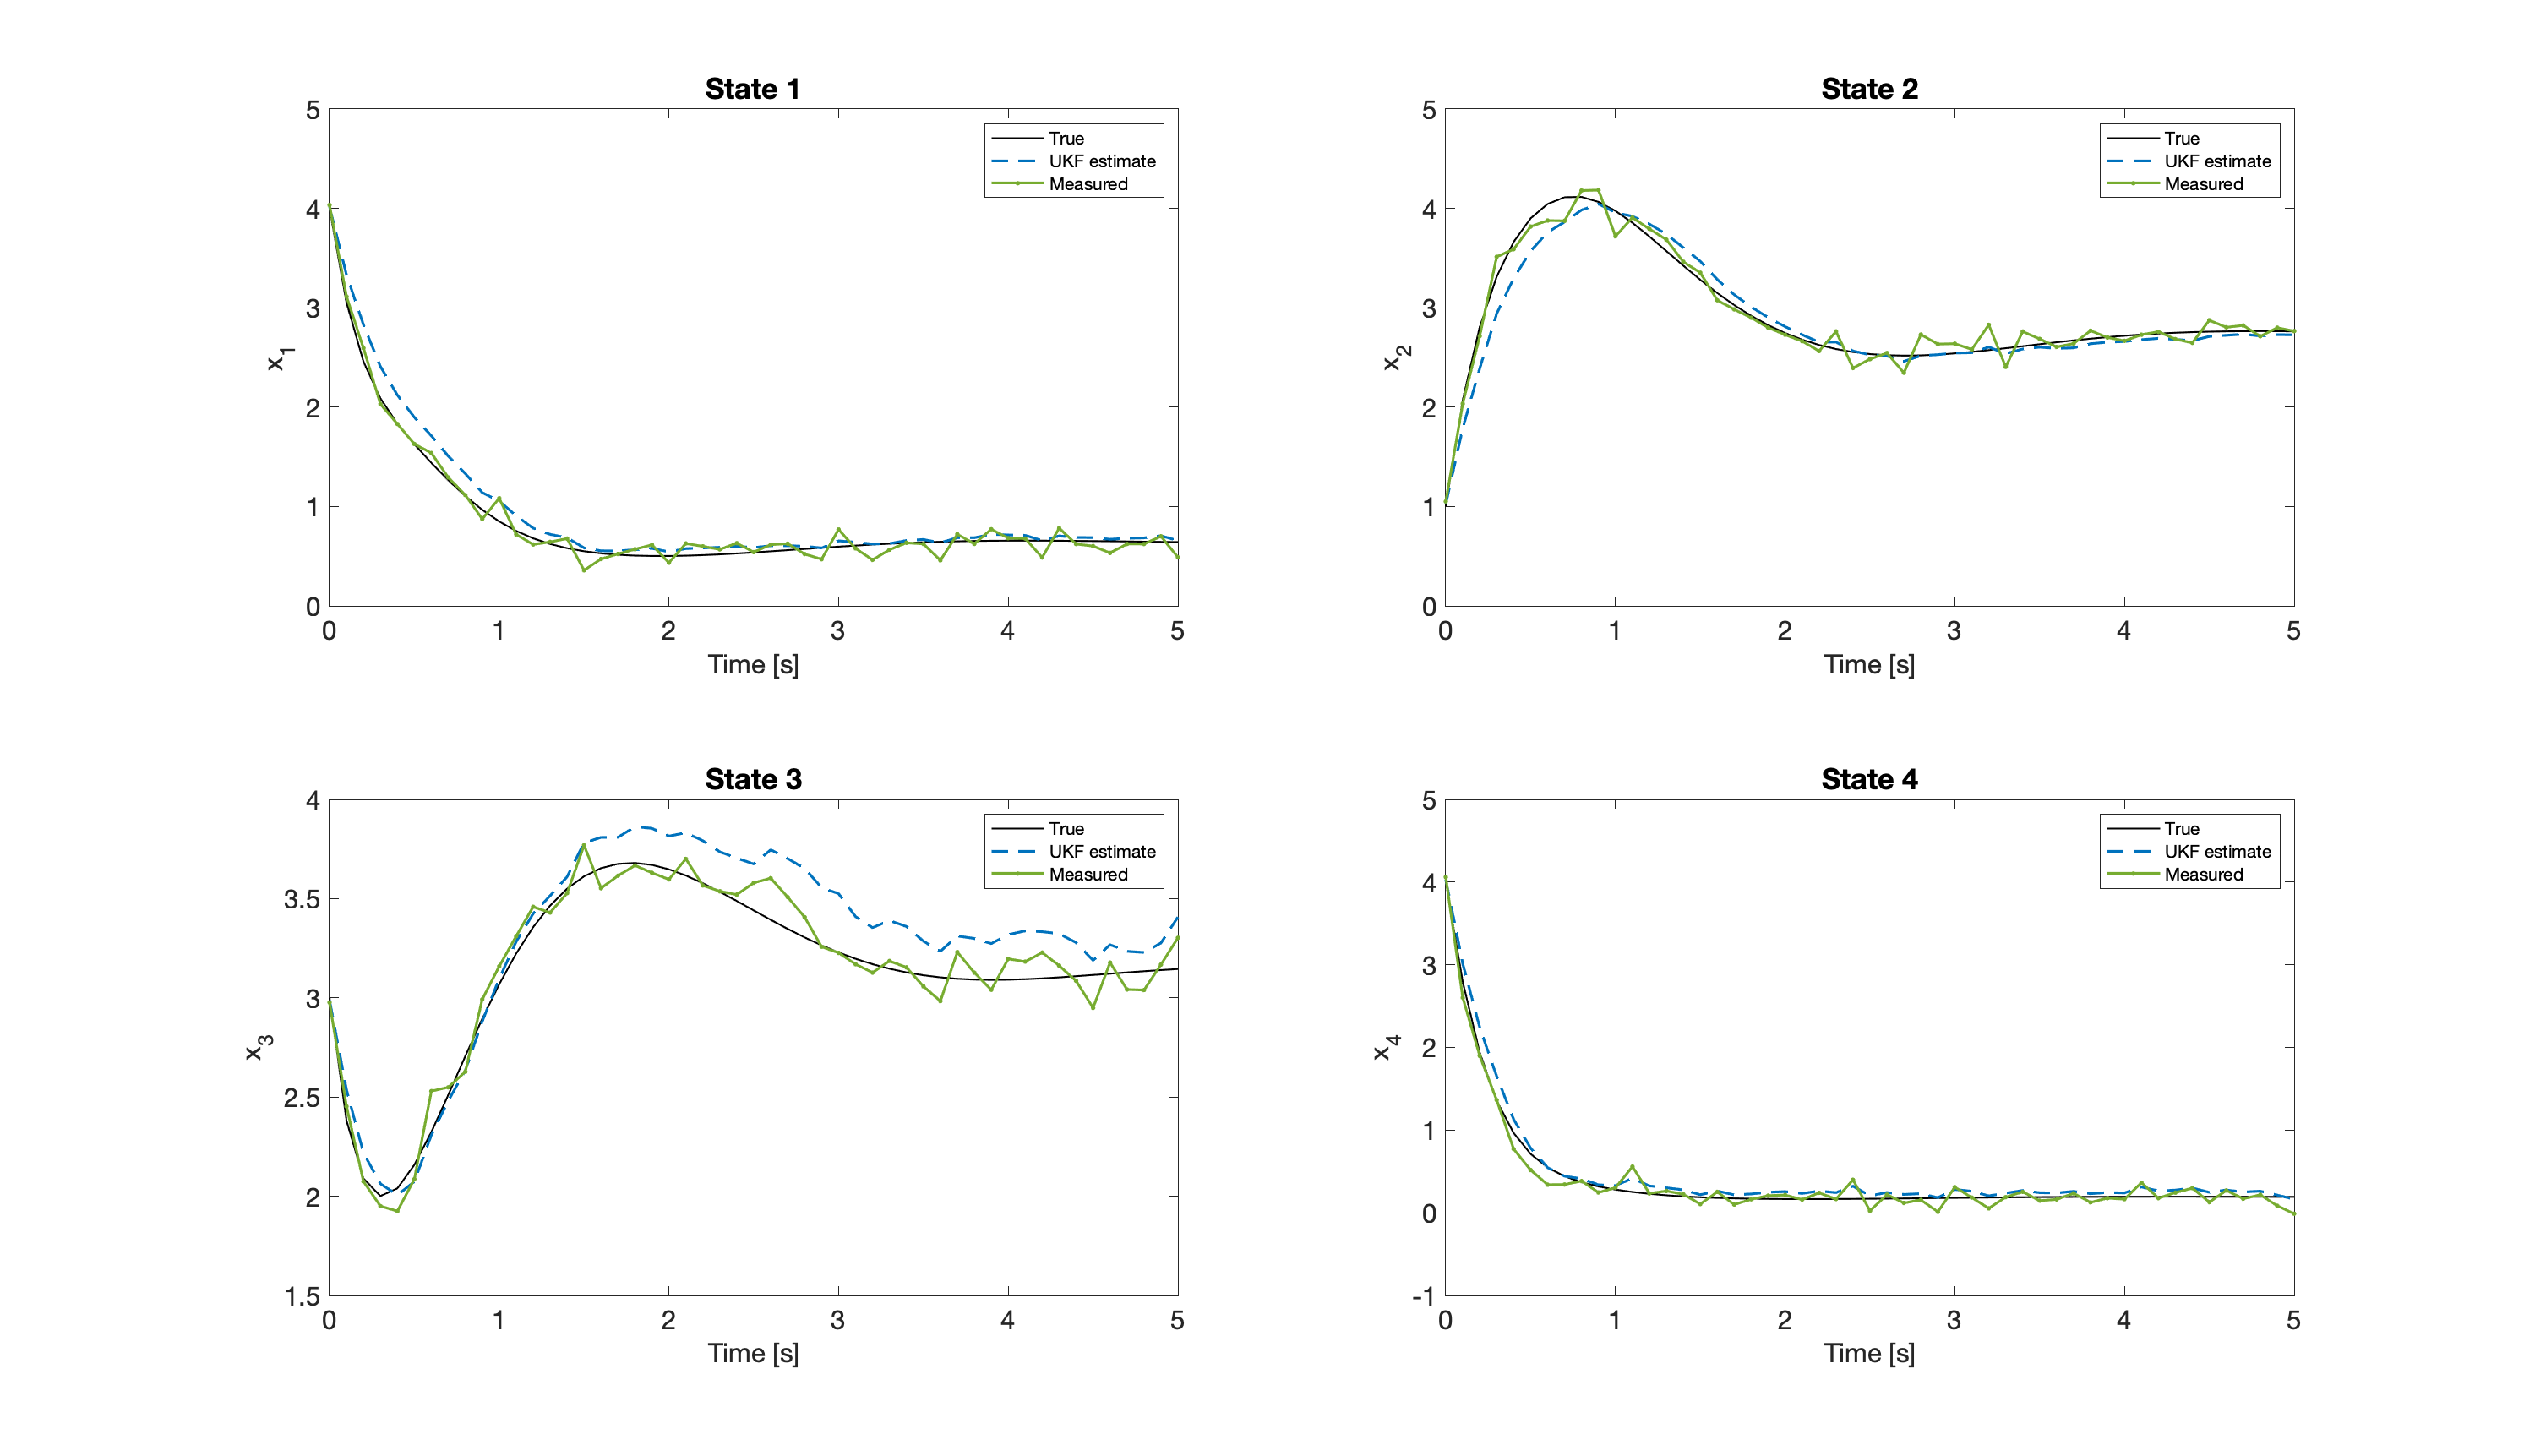
\includegraphics[scale = 0.3]{UKF_states.png}
    \caption{Performance of all four state variables with all four states being corrected. The model is initialized with $x_0 = [4, 1, 3, 4]^T$, which is close to the system's true values and is why the system quickly converges with the true values. The measured and true values are very close together because the system has low values of measurement noise, $R=0.01$, and process noise, $Q=diag([0.2 0.1 0.3 .4 .2 .3 .2 .1])$. The values for $Q$ and $R$ were not taken from the original example \cite{article5}, which is a factor to consider when comparing results.}
    \label{fig:UKF_states}
\end{figure}

\comment{
\noindent An attempt was made to observe how the system changes with differing values of noise. In the real world, measurement noise values of $R=0.01$ is quite low; therefore, there was interest in seeing how increasing this value would change the system's behavior. However, }


\clearpage
\subsubsection{Parameter estimation}

Similar to chapter chapter~\ref{chap:EKF_Meskin}, joint parameter estimation can also be applied to the UKF. This example will be using the exact same dataset for measured and true system values as the one used in the EKF version. In order to estimate parameters, $\alpha_1,\alpha_2, \alpha_3, \alpha_4$, declare them as new states. Recall from the earlier EKF example that the system is as follows
\begin{align*}
\dot x_1 &= x_5  x_3^{g_{13}} x_5^{g_{15}} - \beta_1 x_1^{h_{11}} , \\
\dot x_2 &= x_6  x_1^{g_{21}} - \beta_2 x_2^{h_{22}}, \\
\dot x_3 &= x_7  x_2^{g_{32}} - \beta_3 x_3^{h_{33}} x_4^{h_{34}}, \\
\dot x_4 &= x_8   x_1^{g_{41}} - \beta_4 x_4^{h_{44}} \\
\dot x_5 &= \dot x_6= \dot x_7 = \dot x_8 = 0.
\end{align*}

\noindent The system is initialized with the same values as the EKF four parameter example, with the initial state being $x_0 = [4, 1, 3, 4, 20, 8, 3, 2]^T$ and the state covariance being $P_0 = .01I$. Also, the values of $Q$ and $R$ also remain the same. The results of the UKF on this 8 state system is illustrated in ~\ref{fig:UKF_4param}. Compared with the EKF results, the UKF seems to do poorer for State 3. However, in terms of parameter estimation, the EKF and UKF version seem to have the exact same performance, as shown in ~\ref{tab:UKF_4param}. These results may possibly be adjusted by changing hyper parameter values and can be explored in future work.

\begin{figure}[h]
    \centering
    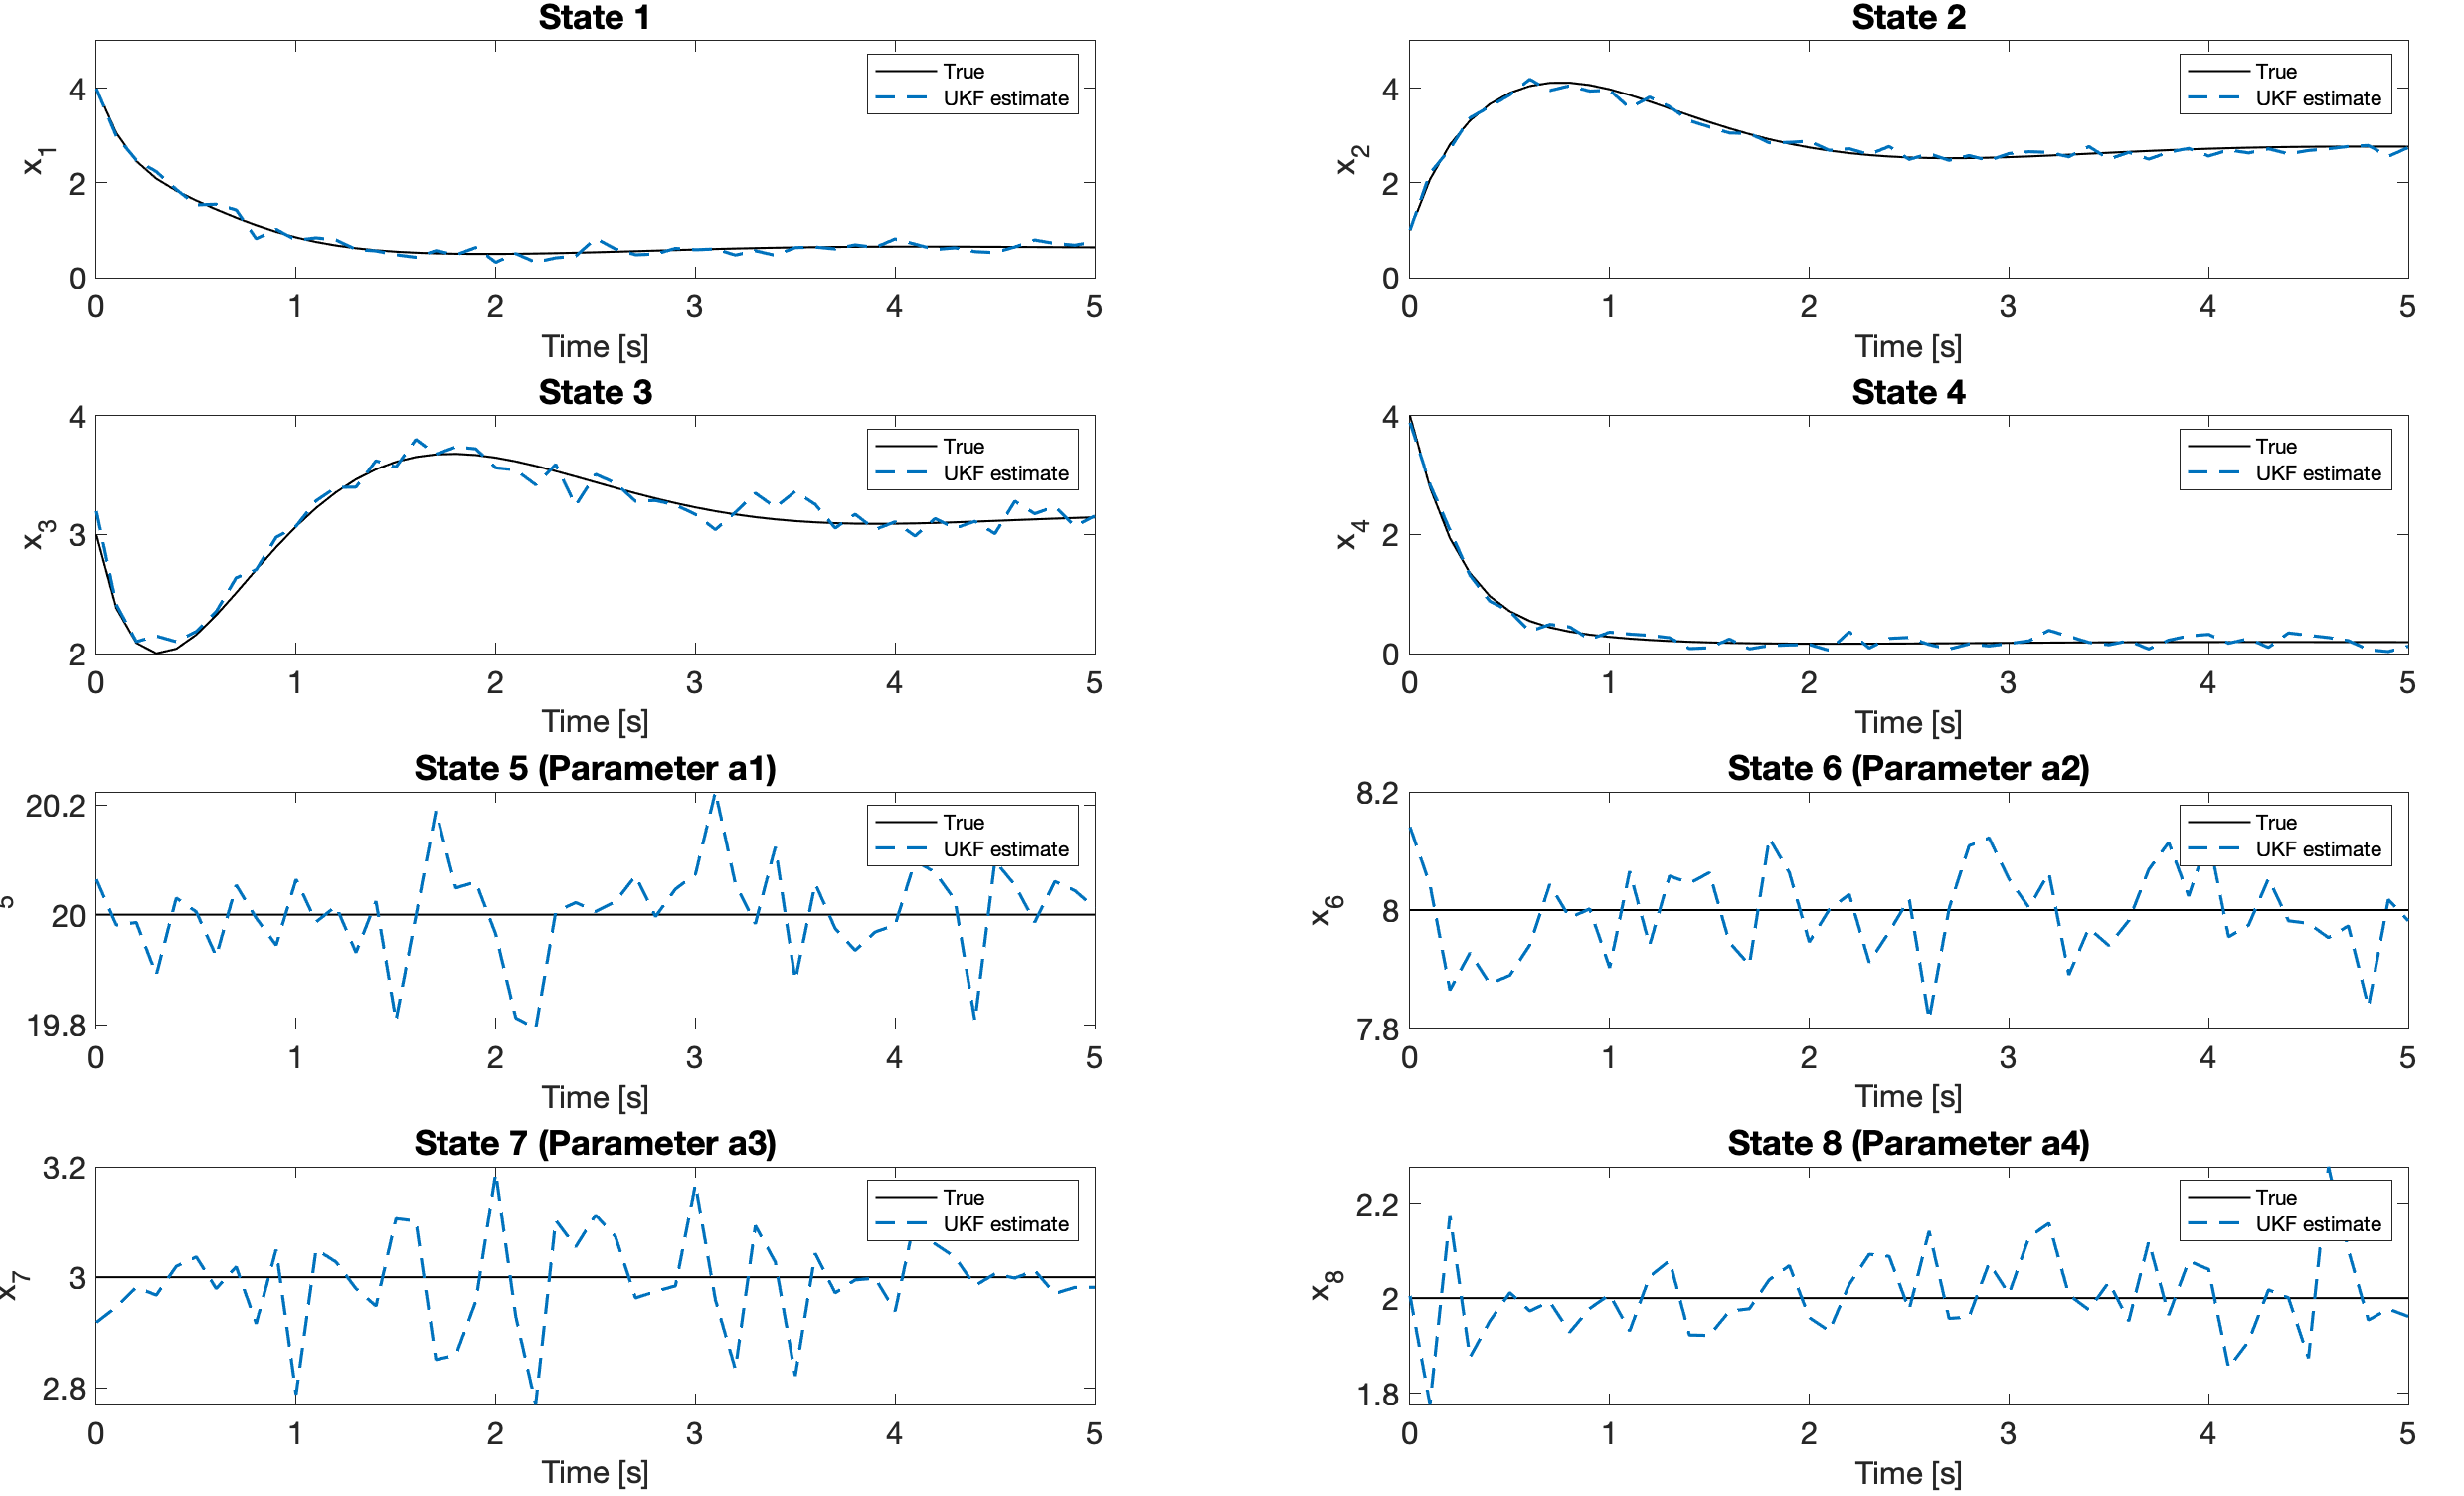
\includegraphics[scale = 0.5]{UKF_4param.png}
    \caption{ds}
    \label{fig:UKF_4param}
\end{figure}

\begin{center}
\begin{table}[h]
\centering
\begin{tabular}{ |P{2cm}||P{1cm} P{2.5cm} P{2.5cm} P{2.5cm} |}
    \hline
    \multicolumn{5}{|c|}{Parameter Values} \\ 
    \hline
     Parameters & True & EKF estimate & UKF estimate &IUKF estimate \\
    \hline
    $\alpha_1$ & 20.0  & 20.0125 &20.0125&19.9744 \\
    $\alpha_2$ & 8.0  & 7.9819  &7.9819& 8.0017 \\
    $\alpha_3$ & 3.0  & 2.9818 &2.9818& 3.0015 \\
    $\alpha_4$ & 2.0 & 1.9614 &1.9614 & 2.0016 \\
    \hline
\end{tabular}
\caption{This table shows the true values of the parameters, the final EKF prediction of the parameters (as a reference to compare filter performance), the final UKF prediction of parameters, and the final IUKF prediction of the parameters. Here, the term final is being used to denote the performance of the filter after 50 time-steps. Interestingly, the performance of the EKF is the exact same as the performance of the UKF. By changing the hyper-parameters for the UKF, the model may be able to provide more accurate results.}
\label{tab:UKF_4param}
\end{table}
\end{center}

\clearpage

\clearpage
\noindent Residuals, also known as the innovation, are one way to access the model's performance. Recall that the residual is the difference between the actual measurement values and the predicted measurement values. Generally, a strong residual graph has

\begin{itemize}
\item a symmetrical distribution that is clustered toward the center,
\item values that are close to 0,
\item a random or unclear pattern.
\end{itemize}

\noindent Figure ~\ref{fig:4params} is the residual graph of the system where the EKF is applied to the four states and four parameters, $\alpha_1, \hdots, \alpha_4$. While this residual graph has values close to 0 and a symmetrical distribution, the pattern is similar to the behavior of the states. Therefore, though UKF can be applied to this nonlinear system, performance can be further optimized.

\begin{figure}[h]
    \centering
    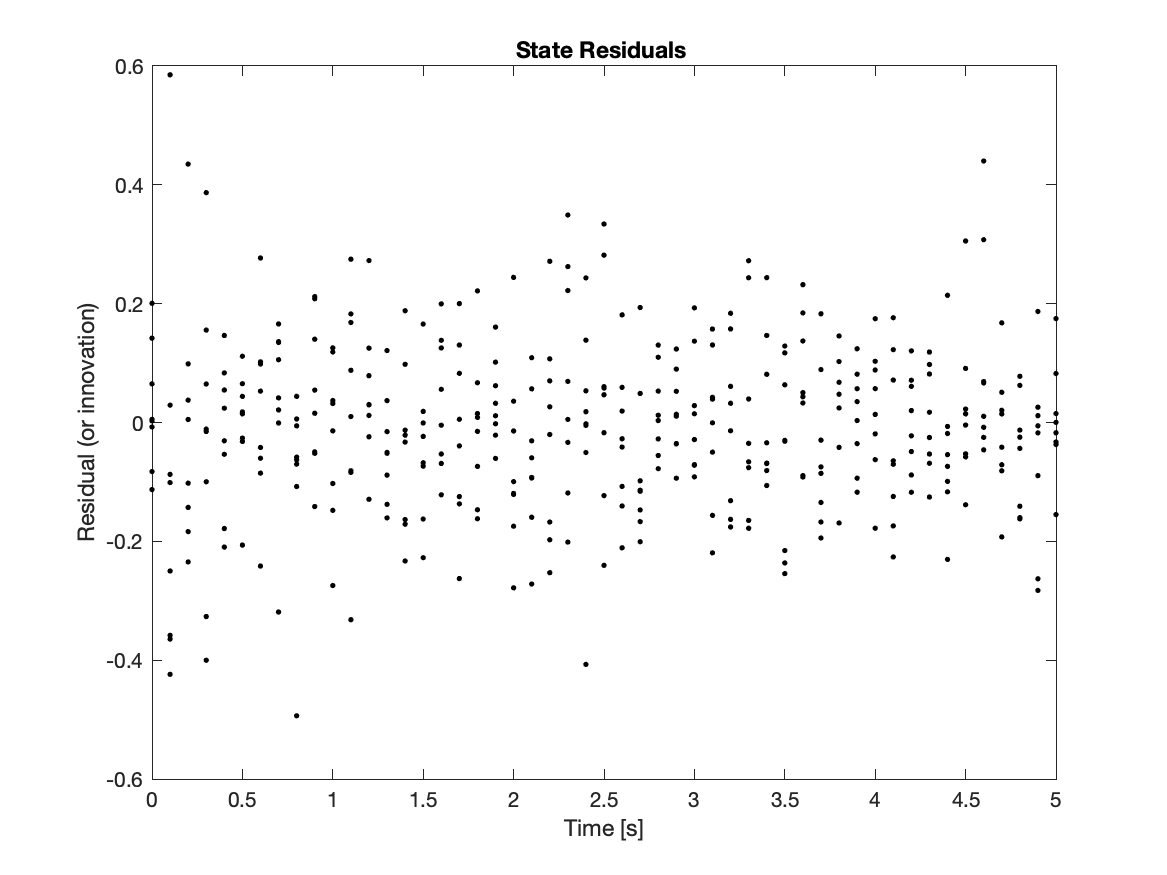
\includegraphics[scale = 0.6]{UKF_4param_residual.png}
    \caption{Built in matlab, four state correction and 4 param}
    \label{fig:4params}
\end{figure}

\noindent Future work includes using the UKF for parameter fitting. One approach would be to use a technique similar to the one employed in chapter 3.2. Alternatively, another non-linear Kalman Filter technique, known as the Dual Unscented Kalman Filter, may also be a promising solution. Either of these two methods will likely be better than the method used in chapter 3.2, because calculating the exponential matrix and jacobian of the system is very computationally expensive and can be avoided with the UKF.

%\noindent \textcolor{red}{Expand here on correcting for 1+ states, currently we are having technical challenges in completing this step}













